% Options for packages loaded elsewhere
\PassOptionsToPackage{unicode}{hyperref}
\PassOptionsToPackage{hyphens}{url}
%
\documentclass[
]{book}
\usepackage{amsmath,amssymb}
\usepackage{lmodern}
\usepackage{ifxetex,ifluatex}
\ifnum 0\ifxetex 1\fi\ifluatex 1\fi=0 % if pdftex
  \usepackage[T1]{fontenc}
  \usepackage[utf8]{inputenc}
  \usepackage{textcomp} % provide euro and other symbols
\else % if luatex or xetex
  \usepackage{unicode-math}
  \defaultfontfeatures{Scale=MatchLowercase}
  \defaultfontfeatures[\rmfamily]{Ligatures=TeX,Scale=1}
\fi
% Use upquote if available, for straight quotes in verbatim environments
\IfFileExists{upquote.sty}{\usepackage{upquote}}{}
\IfFileExists{microtype.sty}{% use microtype if available
  \usepackage[]{microtype}
  \UseMicrotypeSet[protrusion]{basicmath} % disable protrusion for tt fonts
}{}
\makeatletter
\@ifundefined{KOMAClassName}{% if non-KOMA class
  \IfFileExists{parskip.sty}{%
    \usepackage{parskip}
  }{% else
    \setlength{\parindent}{0pt}
    \setlength{\parskip}{6pt plus 2pt minus 1pt}}
}{% if KOMA class
  \KOMAoptions{parskip=half}}
\makeatother
\usepackage{xcolor}
\IfFileExists{xurl.sty}{\usepackage{xurl}}{} % add URL line breaks if available
\IfFileExists{bookmark.sty}{\usepackage{bookmark}}{\usepackage{hyperref}}
\hypersetup{
  pdftitle={Sozialwissenschaftliche Datenanalyse mit R},
  pdfauthor={Kenneth Horvath \& Guy Schwegler},
  hidelinks,
  pdfcreator={LaTeX via pandoc}}
\urlstyle{same} % disable monospaced font for URLs
\usepackage{color}
\usepackage{fancyvrb}
\newcommand{\VerbBar}{|}
\newcommand{\VERB}{\Verb[commandchars=\\\{\}]}
\DefineVerbatimEnvironment{Highlighting}{Verbatim}{commandchars=\\\{\}}
% Add ',fontsize=\small' for more characters per line
\usepackage{framed}
\definecolor{shadecolor}{RGB}{248,248,248}
\newenvironment{Shaded}{\begin{snugshade}}{\end{snugshade}}
\newcommand{\AlertTok}[1]{\textcolor[rgb]{0.94,0.16,0.16}{#1}}
\newcommand{\AnnotationTok}[1]{\textcolor[rgb]{0.56,0.35,0.01}{\textbf{\textit{#1}}}}
\newcommand{\AttributeTok}[1]{\textcolor[rgb]{0.77,0.63,0.00}{#1}}
\newcommand{\BaseNTok}[1]{\textcolor[rgb]{0.00,0.00,0.81}{#1}}
\newcommand{\BuiltInTok}[1]{#1}
\newcommand{\CharTok}[1]{\textcolor[rgb]{0.31,0.60,0.02}{#1}}
\newcommand{\CommentTok}[1]{\textcolor[rgb]{0.56,0.35,0.01}{\textit{#1}}}
\newcommand{\CommentVarTok}[1]{\textcolor[rgb]{0.56,0.35,0.01}{\textbf{\textit{#1}}}}
\newcommand{\ConstantTok}[1]{\textcolor[rgb]{0.00,0.00,0.00}{#1}}
\newcommand{\ControlFlowTok}[1]{\textcolor[rgb]{0.13,0.29,0.53}{\textbf{#1}}}
\newcommand{\DataTypeTok}[1]{\textcolor[rgb]{0.13,0.29,0.53}{#1}}
\newcommand{\DecValTok}[1]{\textcolor[rgb]{0.00,0.00,0.81}{#1}}
\newcommand{\DocumentationTok}[1]{\textcolor[rgb]{0.56,0.35,0.01}{\textbf{\textit{#1}}}}
\newcommand{\ErrorTok}[1]{\textcolor[rgb]{0.64,0.00,0.00}{\textbf{#1}}}
\newcommand{\ExtensionTok}[1]{#1}
\newcommand{\FloatTok}[1]{\textcolor[rgb]{0.00,0.00,0.81}{#1}}
\newcommand{\FunctionTok}[1]{\textcolor[rgb]{0.00,0.00,0.00}{#1}}
\newcommand{\ImportTok}[1]{#1}
\newcommand{\InformationTok}[1]{\textcolor[rgb]{0.56,0.35,0.01}{\textbf{\textit{#1}}}}
\newcommand{\KeywordTok}[1]{\textcolor[rgb]{0.13,0.29,0.53}{\textbf{#1}}}
\newcommand{\NormalTok}[1]{#1}
\newcommand{\OperatorTok}[1]{\textcolor[rgb]{0.81,0.36,0.00}{\textbf{#1}}}
\newcommand{\OtherTok}[1]{\textcolor[rgb]{0.56,0.35,0.01}{#1}}
\newcommand{\PreprocessorTok}[1]{\textcolor[rgb]{0.56,0.35,0.01}{\textit{#1}}}
\newcommand{\RegionMarkerTok}[1]{#1}
\newcommand{\SpecialCharTok}[1]{\textcolor[rgb]{0.00,0.00,0.00}{#1}}
\newcommand{\SpecialStringTok}[1]{\textcolor[rgb]{0.31,0.60,0.02}{#1}}
\newcommand{\StringTok}[1]{\textcolor[rgb]{0.31,0.60,0.02}{#1}}
\newcommand{\VariableTok}[1]{\textcolor[rgb]{0.00,0.00,0.00}{#1}}
\newcommand{\VerbatimStringTok}[1]{\textcolor[rgb]{0.31,0.60,0.02}{#1}}
\newcommand{\WarningTok}[1]{\textcolor[rgb]{0.56,0.35,0.01}{\textbf{\textit{#1}}}}
\usepackage{longtable,booktabs,array}
\usepackage{calc} % for calculating minipage widths
% Correct order of tables after \paragraph or \subparagraph
\usepackage{etoolbox}
\makeatletter
\patchcmd\longtable{\par}{\if@noskipsec\mbox{}\fi\par}{}{}
\makeatother
% Allow footnotes in longtable head/foot
\IfFileExists{footnotehyper.sty}{\usepackage{footnotehyper}}{\usepackage{footnote}}
\makesavenoteenv{longtable}
\usepackage{graphicx}
\makeatletter
\def\maxwidth{\ifdim\Gin@nat@width>\linewidth\linewidth\else\Gin@nat@width\fi}
\def\maxheight{\ifdim\Gin@nat@height>\textheight\textheight\else\Gin@nat@height\fi}
\makeatother
% Scale images if necessary, so that they will not overflow the page
% margins by default, and it is still possible to overwrite the defaults
% using explicit options in \includegraphics[width, height, ...]{}
\setkeys{Gin}{width=\maxwidth,height=\maxheight,keepaspectratio}
% Set default figure placement to htbp
\makeatletter
\def\fps@figure{htbp}
\makeatother
\setlength{\emergencystretch}{3em} % prevent overfull lines
\providecommand{\tightlist}{%
  \setlength{\itemsep}{0pt}\setlength{\parskip}{0pt}}
\setcounter{secnumdepth}{5}
\usepackage{booktabs}
\usepackage{amsthm}
\makeatletter
\def\thm@space@setup{%
  \thm@preskip=8pt plus 2pt minus 4pt
  \thm@postskip=\thm@preskip
}
\makeatother
\ifluatex
  \usepackage{selnolig}  % disable illegal ligatures
\fi
\usepackage[]{natbib}
\bibliographystyle{apalike}

\title{Sozialwissenschaftliche Datenanalyse mit R}
\author{Kenneth Horvath \& Guy Schwegler}
\date{HS 2021}

\begin{document}
\maketitle

{
\setcounter{tocdepth}{1}
\tableofcontents
}
\hypertarget{einfuxfchrung}{%
\chapter*{Einführung}\label{einfuxfchrung}}
\addcontentsline{toc}{chapter}{Einführung}

Das Seminar ``Sozialwissenschaftliche Datenanalyse mit R'' bietet eine systematische Einführung in das Statistikpaket R sowie die Benutzeroberfläche RStudio. R ist eine Open Source Software, die sich unter anderem durch Flexibilität sowie durch vielfältige Möglichkeiten der numerischen und grafischen Datenanalyse auszeichnet. Das Seminar führt auf der einen Seite allgemein in den Aufbau des Programms und dessen Funktionsweisen ein. Auf der anderen Seite werden gewisse statistische Verfahren auch in inhaltliche Abstimmung mit der Vorlesung ``Grundlagen der multivariaten Statistik'' vermittelt. Anhand der Funktionsweisen und der Verfahren werden dann Techniken des effizienten Datenmanagements, Möglichkeiten zur eigenständigen Programmierung von kleinen Funktionen sowie Formen der grafischen Datenanalyse und Ergebnisdarstellung besprochen.

Das vorliegende Dokument ist ein sogenanntes Bookdown \citep{R-bookdown}, siehe auch \href{https://bookdown.org/}{hier}, und dient der Ergebnissicherung im Seminarverlauf. Das heisst dass die im Seminar besprochene Themen hiernochmals schriftlich festgehalten, diskutiert und allenfalls mit Literatur ergänzt werden (siehe für allgemeine Literatur etwa \citet{DiazBone2019}, \citet{Kabacoff2015} oder \citet{Manderscheid2017}). Das Bookdown wird laufend aktualisiert. Ebenfalls werden in diesem Bookdown die Lösungen für die im Seminar beziehungsweise in den Wochenplänen gestellten Aufgaben präsentiert (Falllösungen).

\hypertarget{wocheplan-01}{%
\chapter{Wocheplan 01}\label{wocheplan-01}}

\ldots Vorbereitung von der 01. auf die 02.Einheit.

\hypertarget{sozialwissenschaftliche-datenanalyse}{%
\section{Sozialwissenschaftliche Datenanalyse}\label{sozialwissenschaftliche-datenanalyse}}

Das Seminar ``sozialwissenschaftliche Datenanalyse mit R'' versucht eine Realität des statistischen Arbeitens zu vermitteln und ergänzt so die Vorlesung ``Grundlagen der multivariaten Statistik'' gleich in zweierlei Hinsicht: Erstens wird eine Auswahl der gelernten statistischen Verfahren konkret angewendet (und so auch nochmals repetiert). Zweitens zeigt sich neben den eigentlichen Verfahren ein weiterer, impliziter Teil der Statistik: ein Umgang mit Daten, deren Aufbereitung und Verarbeitung sowie die damit einhergehenden Herausforderungen.

Hinter dem Seminar steht eine bestimmte Vorstellung der sozialwissenschaftlichen Datenanalyse, die folgende Teile enthält \citep{WickhamGrolemund2016}:
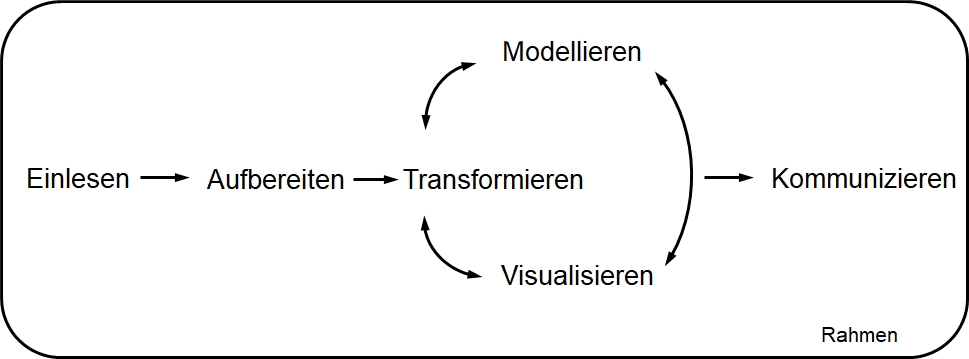
\includegraphics{Bilder/Modell.jpg}

Als erster Schritt müssen die Daten eingelesen bzw. \textbf{importiert} werden. Die importierten Daten gilt es dann \textbf{aufzubereiten} und aufzuräumen. Das bedeutet, dass sie in einer konsistenten Form gespeichert werden sollen (z.Bsp. dass jede Zeile einer Person und jede Spalte einer Variable entspricht). Dieser zweite Schritt ist im Rahmen von Sekundärdaten (wie auch wir sie verwenden werden) oft bereits erfolgt. Ein weiterer Schritt ist es dann, die Daten zu \textbf{transformieren}. Das heisst die Fälle und ihre Ausprägungen werden auf ein bestimmes Interesse eingegrenzt (z.Bsp. auf alle Personen die über ein bestimmtes Einkommen verfügen), neue Variablen werden erstellt (die Funktionen bestehender Variablen sind, etwa Einkommensklassen), und eine Reihe von zusammenfassenden Statistiken werden berechnet (verschiedene univariate Kennwerte). Das Aufbereiten und Transformieren ist ein grosser Teil der statistischen Analyse \citep[es ist ein Kampf mit den Daten,][Kap.1.1]{WickhamGrolemund2016}. Ziel dieser Arbeit ist es, die Daten in eine passende Form zu bringen, um optimal mit ihnen arbeiten zu können.

Wenn die Daten (voerst) in einer optimalen Form vorliegen gibt es zwei Hauptmotoren der Wissensgenerierung \citep[Kap.1.1]{WickhamGrolemund2016}: Visualisierung und Modellierung. Mit \textbf{Visualisierungen} lässt sich schnell eine Übersicht gewinnen (z.Bsp. könnte es überhaupt einen Zusammenhang zwischen zwei Variablen geben?). \textbf{Modellierungen} wiederum ergänzen diese ersten Einsichten, indem präzise Antworten auf Fragen möglich sind (wie gross ist der Zusammenhang genau?).

Das Transformieren, Visualisieren und Modellieren der Daten ist dabei keineswegs ein linearer Prozess, sondern es ergeben sich in ihm immer wieder Wechselwirkungen, Rückbezüge und dadurch neue Wege, um an die Daten heranzutreten. Der letzte Schritt der Datenanalyse ist die \textbf{Kommunikation}. Es gilt also sowohl das Vorgehen (zumindest teilweise) als inbesondere auch die Ergebnisse der Analyse anderen mitzuteilen.

Diese Prozesse der Datenanalyse finden alle in einem bestimmen \textbf{Rahmen} statt \citep[vgl. auch][3]{Sauer2019}. Dies ist auf der einen Seite die Idees des Programmierens im Vorgehen selber \citep[vgl.][Kap.1.1]{WickhamGrolemund2016}. Auf der anderen Seite bilden aber die Sozialwissenschaften selber auch einen Rahmen, anhand dessen etwa Datenstrukturen (z.Bsp. dass eine Person ein Fall und damit eine Zeile ist) oder angemessene Ziele der Analyse (ab wann ist ein Zusammenhang etwa ``gross''?) vorgegeben werden.

\hypertarget{ziel-des-kurses}{%
\section{Ziel des Kurses}\label{ziel-des-kurses}}

Das Seminar verfolgt zwei miteinander verzahnte, übergeordnete Lernziele. Einerseits sollen die Studierenden sich Grundkenntnisse der statistischen Datenanalyse mit R aneignen. Andererseits werden ausgewählte Inhalte der Vorlesung praktisch angewandt und damit auch veranschaulicht.\footnote{Die zwei miteinander verzahnte Lernziele führen auch dazu, dass das Seminar allerdings nicht als eigentliche Übung zur Vorlesung funktioniert (und das nicht alle Inhalte der Vorlesung im Seminar behandelt werden können).}

Konkret sollen die Studierenden am Ende des Semesters\ldots{}

\begin{itemize}
\tightlist
\item
  \ldots einen ersten Einblick in Abläufe und Anforderungen softwaregestützter Datenanalyse haben,
\item
  \ldots typische Herausforderungen statistischen Arbeitens eigenständig bewältigen können,
\item
  \ldots die allgemeine Funktionsweise und die Struktur von R verstehen,
\item
  \ldots die Umsetzung ausgewählter multivariater Verfahren in R beherrschen,
\item
  \ldots dabei auch grafische Verfahren als zentrale Bausteine aktueller Datenanalyse einsetzen können
\item
  \ldots sowie die Grundlage dafür erworben haben, flexibel eigene Analysestrategien in R umzusetzen.
\end{itemize}

\hypertarget{r-als-programm-rstudio}{%
\section{R als Programm \& RStudio}\label{r-als-programm-rstudio}}

R als Programmiersprache wurde von Beginn an für die Statistik beziehungsweise für die Statistiklehre entwickelt. Die Anfänge des Programms fanden in den 1990er Jahre an der Universität Auckland in Neuseeland statt, wo R von Ross Ihaka und Robert Gentleman entwickelt wurde \citep[1]{Manderscheid2017}. Der Buchstabe ``R'' als Name geht sowohl auf eine ältere Grundlage zurück -- die Programmiersprache ``S'' -- als auch auf die Vornamen der beiden Entwickler \citep[ebd., vgl. auch][13f]{Sauer2019}. Das R-Projekt wurde in der Zusammenareit mit weiteren Wissenschaftler\_Innen voran getrieben und bald auch unter der General Public Licence (\href{https://en.wikipedia.org/wiki/GNU}{GNU}) veröffentlicht \citep[1]{Manderscheid2017}. R ist daher frei zugänglich, kostenlos und darf von allen verändert werden. Es ist insbesondere auch diese \emph{Open Source} Idee, die R zu seiner Verbreitung half -- und die sicherstellt, dass die neusten Entwicklungen in und mit der Software stattfinden.

R als Programm ist in Paketen organisiert und präsentiert sich als ``Statistikumgebung'' \citep[1]{Manderscheid2017}. Ausgehend von der Basisversion bzw. des Basispaketes kann R beliebig erweitert werden. Unter \url{https://cran.r-project.org/} findet sich eine beständig wachsende und umfangreiche Sammlung von Paketen, die sowohl Lösungen für allgemeine Verfahren anbieten (etwa Pakete für die multiple Korrespondenzanalyse, siehe ``soc.ca'') als auch für spezifische Probleme (etwa für ``Atomic Force Microscope Image Analysis'' beim Paket ``AFM''). Diese Pakete können installiert werden und es gilt sie dann jeweils noch zu laden, bevor sie verwendet werden können. Nach dem Beenden des Programms werden die verwendeten Pakete wieder ``versorgt'' und es gilt sie beim nächsten Mal erneut zu laden (die Pakete beleiben aber installiert). Letzterer Vorgang stellt sicher, dass R ``schlank'' bleibt, d.h. nur immer die benötigen Dinge auch ausgeführt werden.

\begin{Shaded}
\begin{Highlighting}[]
\FunctionTok{install.packages}\NormalTok{(}\StringTok{"soc.ca"}\NormalTok{) }\CommentTok{\#...installiert das Paket}
\FunctionTok{library}\NormalTok{(soc.ca) }\CommentTok{\#...lädt das Paket}
\end{Highlighting}
\end{Shaded}

Neben dieser \emph{Open Source} Idee und der daraus folgenden, beständigen Aktualisierung und Erweiterungen des Programms zeichnet R sich weiter durch dessen Stärke im Bereich der Visualisierung aus. Es bieten sich unbegrenzte Möglichkeiten für Grafiken und Diagramme, sowohl bereits in der Basisversion als insbesondere auch mit spezifischen Paketen \citep[siehe][]{R-ggplot2}.

Neben der Basisversion von R und R als eigentlicher Programmiersprache gibt es grafische Benutzeroberflächen (GUIs), um mit der Programmiersprache umzugehen. Im Zentrum unseres Seminars steht \textbf{RStudio}, die am weitesten verbreitete grafische Benutzeroberfläche von R. Diese Oberfläche bietet einige praktische Zusatzfunktionen und erleichtert so das Arbeiten mit R durch Autovervollständigkeitsfunktionen, automatische Einrückungen, Syntaxhervorhebung, integrierte Hilfsfunktion, Informationen zu Objekten im Workspace, menügestützten Oberflächen und Daten-Viewer \citep[18]{Manderscheid2017}. Die eigentliche Arbeit verrichtet aber weiterhin R selber,
und R wird automatisch gestartet wird, wenn Sie RStudio starten \citep[21]{Sauer2019}. Man kann diese Arbeitsteilung mit einem Auto vergleichen: R ist der Motor des Autos, während RStudio das Amaturenbrett ist, vor dem Sie sitzen und das Auto lenken.

\hypertarget{lernziele-der-ersten-woche}{%
\section{Lernziele der ersten Woche}\label{lernziele-der-ersten-woche}}

Die erste Seminarwoche dient dazu, die technischen Voraussetzungen für die gemeinsame Arbeit im Seminar zu prüfen und mit der geplanten Arbeitsweise vertraut zu werden.

Das Seminar zielt nicht nur auf einen Frontalunterricht ab, sondern ist als eine Art ``flipped classroom'' konzipiert. Sie bekommen also von Woche zu Woche konkrete Arbeitsaufträge (die Falllösungen). Diese sollen Sie eigenständig bewältigen und alle Probleme und Unklarheiten notieren, die sich im Arbeitsprozess ergeben. Die gemeinsamen Sitzungen dienen dann dazu, Lösungswege zu den Aufgaben zu präsentieren, offene Fragen zu klären, Konzepte vertiefend zu erläutern und die nächsten Schritte vorzubereiten.

Für jede Woche werden Lernziele und Arbeitsaufträge definiert. Für die erste Seminarwoche lassen sich als Lernziele festhalten:

\begin{itemize}
\tightlist
\item
  Sie wissen, wie Sie die aktuellen Versionen von R und RStudio auf Ihrem Computer installieren
\item
  Sie wissen, wie man R-Pakete installiert und in R lädt
\item
  Sie können eine Funktion aufrufen
\item
  Sie haben einen soliden ersten Eindruck, wie man mit R kommuniziert und einfache Operationen durchführt
\item
  Sie haben eine erste Orientierung zu Unterstützungsangeboten, die man online findet (auch wenn diese teilweise noch überfordernd wirken)
\end{itemize}

\hypertarget{aufgaben-der-ersten-woche}{%
\section{Aufgaben der ersten Woche}\label{aufgaben-der-ersten-woche}}

\begin{enumerate}
\def\labelenumi{\arabic{enumi})}
\item
  Installieren Sie die aktuellen Versionen von R und RStudio auf Ihrem Endgerät! Sie sollten sich Notizen machen, wenn es Probleme gibt -- und für das nächste Mal gleich festhalten, wie Sie diese gelöst haben. Da die Details der Installation vom Betriebssystem und den Spezifikationen des Endgeräts abhängen, ist es normal, dass dieser Prozess manchmal erst auf den zweiten Versuch funktioniert.
\item
  Installieren Sie das Paket ``swirl'' und laden Sie es. ``swirl'' ist eine in R implementierte interaktive Einführung in die Grundlagen von R!
\item
  Rufen Sie die Funktion \texttt{swirl()} auf und spielen Sie ein wenig damit. Rufen Sie sich in Erinnerung, was Sie aus dem letzten Semester noch über die Arbeit mit R wissen! Notieren Sie sich, was Ihnen Sie noch kennen, was Ihnen neu vorkommt, und so weiter.
\item
  Verwenden Sie ein wenig Zeit darauf, online nach R Tutorials, Foren, etc. zu suchen. Halten Sie die URLs von Seiten und Ressourcen fest, die Ihnen hilfreich und/oder wichtig vorkommen (aber unter Umständen noch etwas schwer zu durchschauen) !
\end{enumerate}

Erstellen Sie aus Ihren Notizen ein PDF Dokument (Sie müssen in der ersten Woche noch keinen R Code abgeben), beschriften Sie dieses mit FL01\_NameVorname.pdf und geben das Dokument via OLAT vor der nächsten Einheit ab.

  \bibliography{book.bib,packages.bib}

\end{document}
